\section{Halt on Reset}
\label{sec:HaltOnReset}

The standard debug specification of RISC-V has Halt-on-Reset feature, and mmRISC-1 supports the standard spec, of course. The feature is controlled by setresethaltreq and clrresethaltreq in DMCONTROL register in DM (Debug Module). Once the  Halt-on-Reset is enabled, the CPU always halts before first instruction execution when CPU reset (by RES\_CPU), unless the feature is disabled by JTAG access or power-on-reset \seqsplit{(RES\_ORG)}.\\\\

Please note that the standard Halt-on-Reset feature is disabled when a power-on-reset \seqsplit{(RES\_ORG)} occurs. This means the CPU starts its running on a power-on-reset, and keeps its running until next CPU reset after enabling Halt-on-Reset via JTAG access. Even if you want to prevent CPU execution just after power-on-reset, for example, in order to erase and write embedded non-volatile memory or in order to download program code to internal RAM, the standard specification can not do that. So, the mmRISC-1 has an alternative Halt-on-Reset feature in addition.\\

Figure \ref{fig:HALTONRESET} shows the feature in mmRISC-1. When there is a negation of \seqsplit{RES\_ORG}, if an input signal \seqsplit{FORCE\_HALT\_ON\_RESET\_REQ} is low, the CPU starts from 1st instruction at reset vector, which is normal operation. \\\\

On the other hand, when there is a negation of RES\_ORG, if the input signal \seqsplit{FORCE\_HALT\_ON\_RESET\_REQ} is high, the CPU halts until receiving a resume command from debug I/F. In the case, \seqsplit{FORCE\_HALT\_ON\_RESET\_ACK} will be asserted to indicate the request is acknowledged. After the acknowledgement, external circuit which requires CPU halt should negate \seqsplit{FORCE\_HALT\_ON\_RESET\_REQ} immediately.\\

You can use this feature for both JTAG debug I/F and cJTAG debug I/F. \\\\

As for 4-wire JTAG I/F, \seqsplit{FORCE\_HALT\_ON\_RESET\_REQ} should be properly created according to external request. Figure \ref{fig:HALTONRESETCTRL} might be a good example. When there is a negation of \seqsplit{RES\_ORG},if \seqsplit{RESET\_HALT\_N}(active-low) is driven at low level, the CPU goes to halt state, and resumes from reset vector after resume command is sent via debug port.\\\\

As for 2-wire cJTAG I/F, a conversion block \seqsplit{CJTAG\_2\_JTAG.v} supports the feature, that is, when there is a negation of \seqsplit{RES\_ORG}, if TMSC is driven to low level, CPU halts until receiving resume command from debugger. Details are described in another section.\\

\begin{figure}[H]
    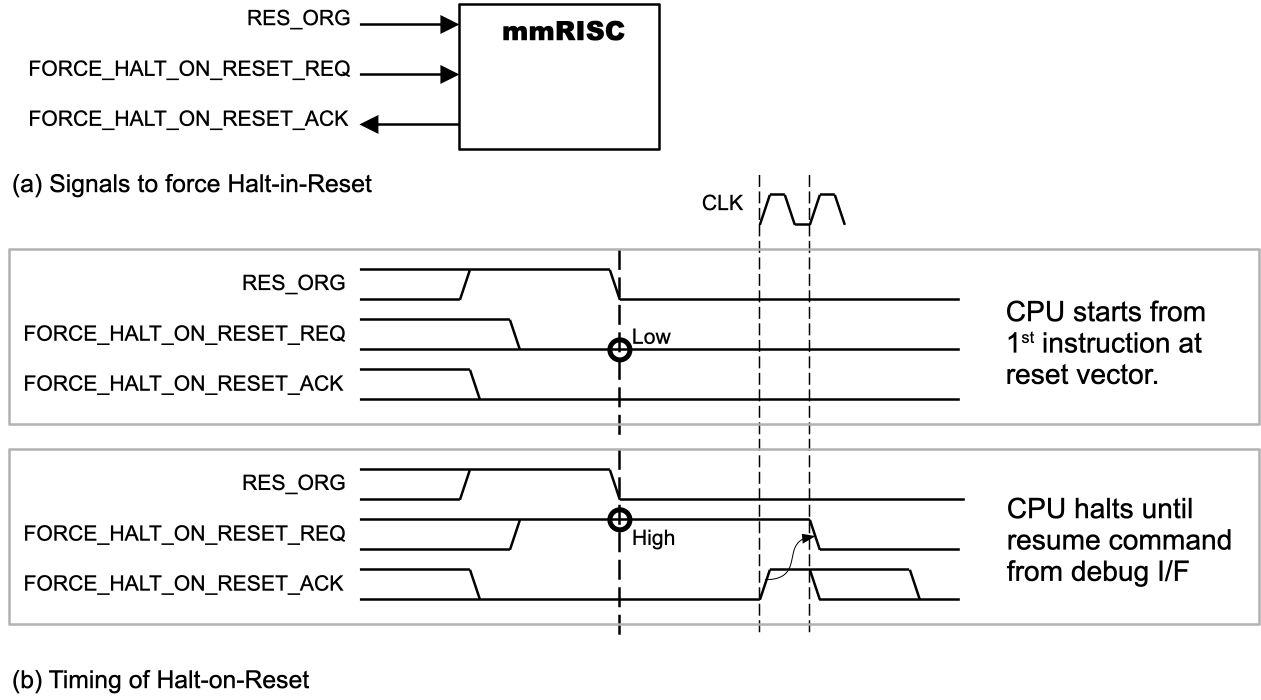
\includegraphics[width=1.00\columnwidth]{./Figure/HaltOnReset_IF.png}
    \caption{Halt on Reset}
    \label{fig:HALTONRESET}
\end{figure}

\begin{figure}[H]
    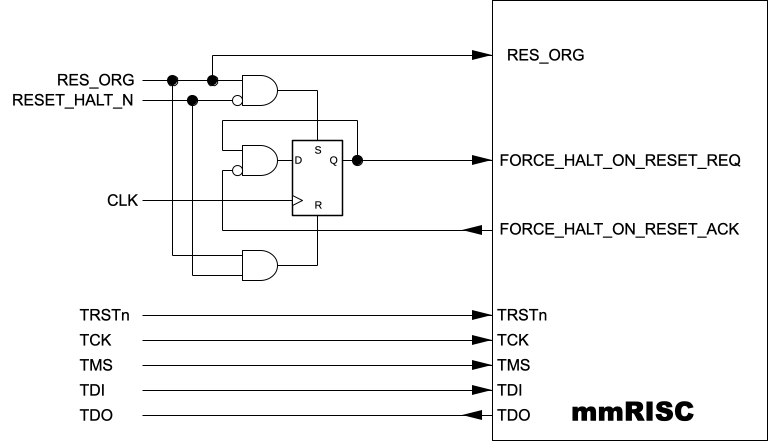
\includegraphics[width=1.00\columnwidth]{./Figure/HaltOnReset_CTRL.png}
    \caption{Example of Control Logic for Halt on Reset}
    \label{fig:HALTONRESETCTRL}
\end{figure}


